\documentclass[
  10pt,     % set default generic font size
  handout   % ignores all the \pause commands
]{beamer}
\usetheme[block=fill]{metropolis}

% -----------------------------------------------------------------------------
% Title and Author Information -- Need to Edit
% -----------------------------------------------------------------------------

\title{H52F-05H: Robust Adaptation to\\Multi-Scale Climate Variability}
\subtitle{Toward Better Water Planning and Management in an Uncertain World I}
\date{14 December 2018}
\author{\alert{James Doss-Gollin}$^1$, David J. Farnham$^2$, Scott Steinschneider$^3$, Upmanu Lall$^1$}
\institute{
  $^1$Columbia University Department of Earth and Environmental Engineering\\
  $^2$Carnegie Institution for Science\\
  $^3$Department of Biological and Environmental Engineering, Cornell University}
\titlegraphic{\hfill\includegraphics[height=1.25cm]{SeasCrown_blue.png}}


% Add footer for AGU
\setbeamertemplate{footline}[text line]{%
  \parbox{0.8\linewidth}{
    \vspace*{-8pt}James Doss-Gollin (\url{james.doss-gollin@columbia.edu})
  }
  \hfill%
  \parbox{0.15\linewidth}{
    \vspace*{-8pt}\raggedleft\insertpagenumber
  }
}

% -----------------------------------------------------------------------------
% Package Configuration -- Don't Necessarily Need to Edit
% -----------------------------------------------------------------------------

% Packages with Options
\usepackage[english]{babel}

% Package List
\usepackage{
  array,                              % for custom table widths
  appendixnumberbeamer,               % don't count appendix slides in progress bar
	booktabs,                           % for better (alternative?) tables
  natbib,                             % references!
	physics,                            % for better notation
  siunitx,                            % for SI notation
  appendixnumberbeamer,               % don't number slides / sections in appendix
}

% cool fonts
\usepackage{fontspec}
\usepackage{fontawesome5}

% figures
\usepackage{graphicx}
\graphicspath{{../fig/}} % can add more

% Fixed-width columns
\usepackage{array}
\newcolumntype{L}[1]{>{\raggedright\let\newline\\\arraybackslash\hspace{0pt}}m{#1}}

% Change the captions
\setbeamerfont{caption}{size=\scriptsize}

% macros
\usepackage{xspace}
\newcommand*{\eg}{e.g.\@\xspace}
\newcommand*{\ie}{i.e.\@\xspace}
\makeatletter
\newcommand*{\etc}{%
    \@ifnextchar{.}%
        {etc}%
        {etc.\@\xspace}%
}
\makeatother
\newcommand{\usd}[1]{\SI[round-precision=2,round-mode=places,round-integer-to-decimal]{#1}[\$]{}}
\newcommand{\normal}{\mathcal{N}}
\newcommand*{\ditto}{---''---}

% Biblatex Setup using a file called library.bib
\setbeamertemplate{bibliography item}[text] % don't print the symbols

% Use the glossaries package
\usepackage[acronym]{glossaries}
\makeglossaries
\newacronym{acc}{ACC}{anthropogenic climate change}
\newacronym{amo}{AMO}{Atlantic Multidecadal Oscillation}
\newacronym{cba}{CBA}{Cost-Benefit Analysis}
\newacronym{enso}{ENSO}{the El Ni\~{n}o-Southern Oscillation}
\newacronym{ffa}{FFA}{flood frequency analysis}
\newacronym{gcm}{GCM}{general circulation model}
\newacronym{hmm}{HMM}{hidden Markov model}
\newacronym{iid}{IID}{independent and identically distributed}
\newacronym{ipcc}{IPCC}{International Panel on Climate Change}
\newacronym{ipo}{IPO}{Interdecadal Pacific Oscillation}
\newacronym{lbda}{LBDA}{living blended drought analysis}
\newacronym{lfv}{LFV}{low-frequency climate variability}
\newacronym{nao}{NAO}{North Atlantic Oscillation}
\newacronym{npv}{NPV}{Net Present Value}
\newacronym{pdo}{PDO}{Pacific Decadal Oscillation}
\newacronym{s2d}{S2D}{seasonal to decadal}
\newacronym{s2s}{S2S}{sub-seasonal to seasonal}

% this has to come last
\usepackage{cleveref}
\usepackage{hyperref}

% -----------------------------------------------------------------------------
% BEGIN DOCUMENT HERE
% -----------------------------------------------------------------------------

\begin{document}

% TITLE PAGE
\maketitle

\begin{frame}{Thanks to...}
  \begin{itemize}
    \item Co-authors
    \begin{itemize}
      \item Upmanu Lall
      \item David J. Farnham
      \item Scott Steinschneider
    \end{itemize}
    \item Funders
    \begin{itemize}
      \item NSF GRPF
      \item Columbia University Fu Foundation SEAS
      \item DoD SERDP
    \end{itemize}
    \item Conveners, colleagues, collaborators
  \end{itemize}
\end{frame}

\begin{frame}{Motivating Example}
  \begin{columns}[T]
    \pause
    \begin{column}{0.5\textwidth}
      \begin{figure}
        \centering
        \caption{
          Permanent structural solution would pose environmental and social impacts and lock in $\approx \$25 \text{billion}$;
          a portfolio of smaller projects may allow a more flexible strategy.
        }
        \includegraphics[width=0.85\columnwidth]{three-barriers.png}\\
        \includegraphics[width=0.85\columnwidth]{flood-concept.png}
      \end{figure}
    \end{column}
    \pause
    \begin{column}{0.5\textwidth}
      \begin{itemize}
        \item ``Because present decisions impact a system's ability to adapt to future needs, flexibility in activating, delaying, and replacing engineering projects should be considered in least‐cost water supply intervention scheduling,'' \citep{erfani:2018}.
        \item How to build a portfolio of risk management investments, over time, given uncertain future climate/society/technology?
      \end{itemize}
    \end{column}
  \end{columns}
\end{frame}

\section{Underlying Ideas}

\begin{frame}{Idea 1: Risk Estimates over Finite Future Periods}
  \begin{alertblock}{Typical Approach:}
    \gls{cba}, probably with discounting, over a \alert{finite} planning horizon of $M$ years (explicitly or implicitly).
  \end{alertblock}
  \begin{columns}
    \pause
    \begin{column}{0.5\textwidth}
      Thus, evaluation of project depends on climate conditions over the next $M$ years:
      \begin{itemize}
        \item For ``mega-project'', $M \geq \SI{50}{years}$
        \item For small, flexible project, $M \leq \SI{5}{years}$
      \end{itemize}
    \end{column}
    \pause
    \begin{column}{0.5\textwidth}
      Misrepresentation of climate risk over $M$ years $\rightarrow$ bias in \gls{cba}
      \includegraphics[width=\textwidth,height=0.5\textheight,keepaspectratio=true]{Bias-Variance-Sketch}
    \end{column}
  \end{columns}
\end{frame}

\begin{frame}{Idea 2: Physical Drivers of Risk Depend on $M$}
  The physical drivers of hazard depend on the projection horizon ($M$).
  \begin{figure}
    \centering
    \includegraphics[width=0.7\textwidth,keepaspectratio=true]{conceptual-sketch-a.png}\\
  \end{figure}
  \pause
  However, our ability to identify these mechanisms depends on information available (\eg, the length of an $N$-year observational record).
  \begin{figure}
    \centering
    \includegraphics[width=0.7\textwidth,keepaspectratio=true]{conceptual-sketch-b.png}
  \end{figure}
\end{frame}

\section{Stylized Experiments}

\begin{frame}{Research Objective}
  \begin{alertblock}{How well can one identify and predict risk}
     associated with cyclical and secular climate signals over a finite design life ($M$),  given limited information (\eg, an $N$-year record).
  \end{alertblock}
  \pause
  In particular, we consider:
  \begin{itemize}
    \item the specific roles of $M$ and $N$;
    \pause
    \item estimation strategy (few processes/parameters $\Rightarrow$ many processes/parameters)
    \pause
    \item the form of the underlying climate signal.
  \end{itemize}
  \pause
  Use simplest possible representation of key processes.
\end{frame}

\begin{frame}{Breathless Overview of Methods}
  \begin{columns}[T]
    \begin{column}{0.475\textwidth}
      We will consider:
      \begin{itemize}
        \item 3 scenarios:
        \begin{itemize}
          \item \gls{lfv} only
          \item linear trend only
          \item trend + \gls{lfv}
        \end{itemize}
        \item 3 fitting models:
        \begin{itemize}
          \item stationary
          \item trend
          \item \gls{hmm}
        \end{itemize}
        \item Many values of $\qty{M, N}$
      \end{itemize}
    \end{column}
    \pause
    \begin{column}{0.475\textwidth}
      \begin{figure}
        \caption{Over- or under-estimating uncertainty leads to biased estimates of $p(X > X^*)$ even if estimate of $X$ is unbiased}
        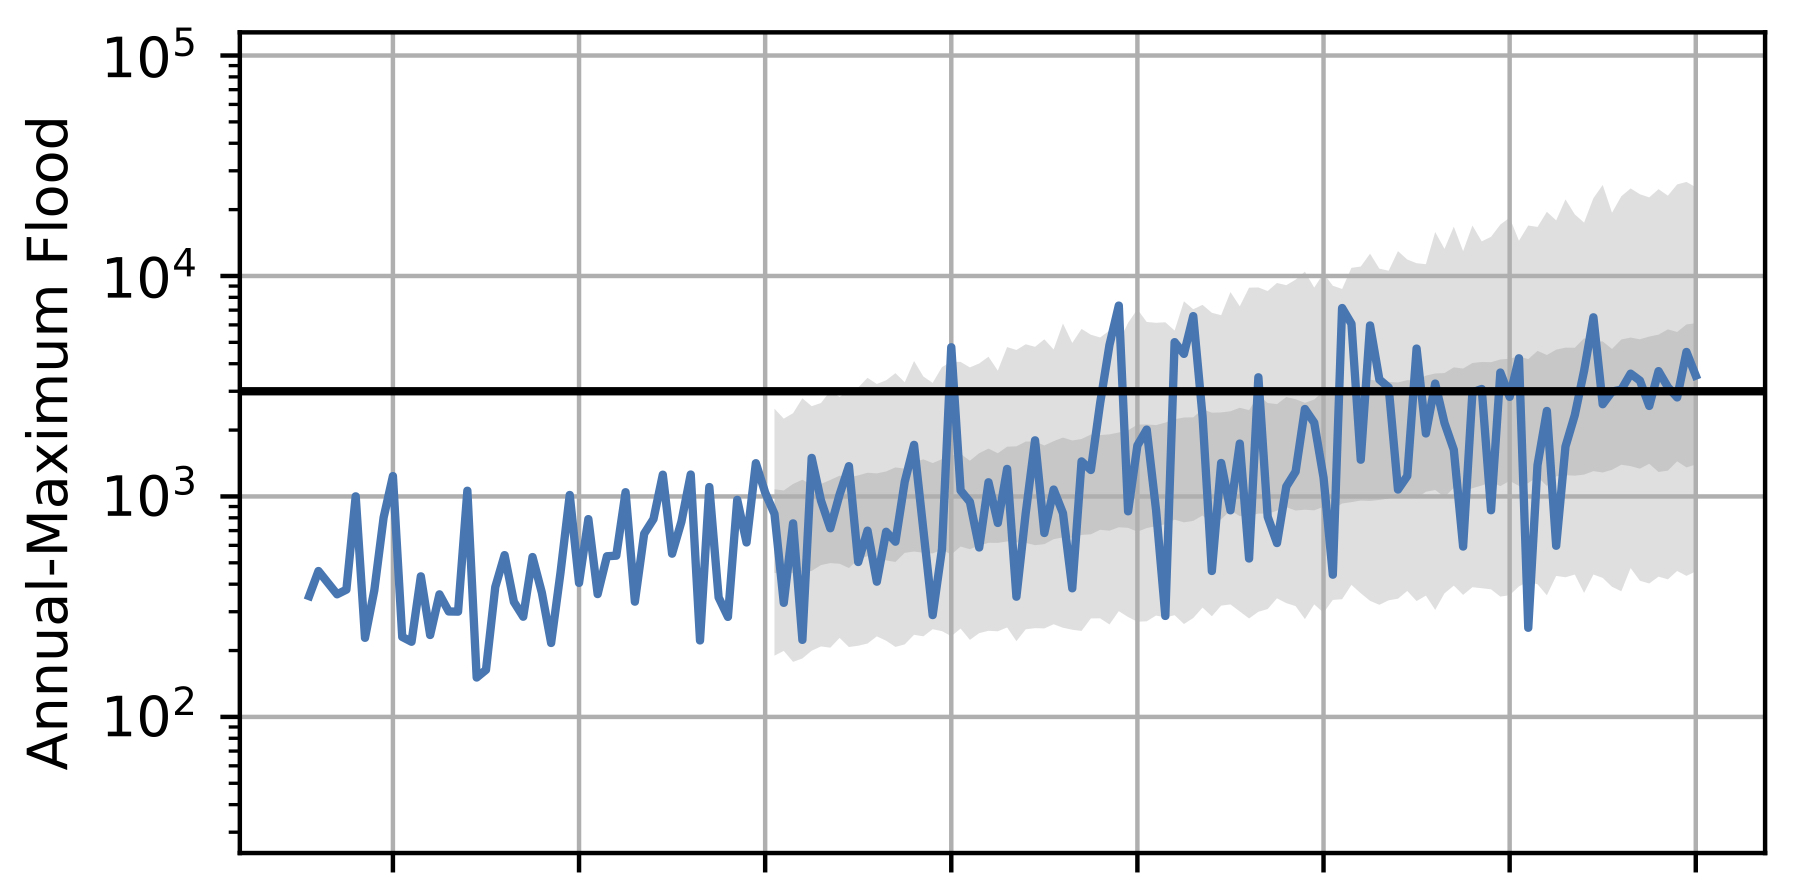
\includegraphics[width=\textwidth]{Example-NINO3-M100-N50-LN2.jpg}
      \end{figure}
      For each combination, use \num{1000} synthetic streamflow sequences to evaluate the expected bias and variance of $p(X > X^*)$
    \end{column}
  \end{columns}
\end{frame}

\begin{frame}{Stationary Scenario (LFV Only)}
  Estimating a trend when none exists may lead to substantial over-estimation of risk, particularly for short $N$ or long $M$.
  Explicitly modeling \gls{lfv} improves estimates, particularly for long $N$.
  \begin{figure}
    \centering
    \includegraphics[width=\textwidth,height=0.625\textheight,keepaspectratio=true]{lfv-only-nino3-bias-variance.pdf}
  \end{figure}
\end{frame}

\begin{frame}{Nonstationary Scenario I (Secular Change Only)}
  For long $M$, it's important to estimate the trend -- but only works well if $N$ also long.
  For short $M$ and short $N$, the uncertainty added by estimating a trend is not worth the bias reduction.
  \begin{figure}
    \centering
    \includegraphics[width=\textwidth,height=0.625\textheight,keepaspectratio=true]{secular-only-nino3-bias-variance.pdf}
  \end{figure}
\end{frame}

\begin{frame}{Nonstationary Scenario II (Secular Change + LFV)}
  Conclusions are similar to ``Secular Change Only'' but variance has increased -- \ie as the system becomes more complex, more data is needed to understand it.
  \begin{figure}
    \centering
    \includegraphics[width=\textwidth,height=0.625\textheight,keepaspectratio=true]{lfv-secular-nino3-bias-variance.pdf}
  \end{figure}
\end{frame}

\section{Discussion}

\begin{frame}{Summary}
  Starting point:
  \begin{enumerate}
    \item Investment evaluation depends on climate condition over finite planning period
    \item Physical drivers of risk depend on planning period
  \end{enumerate}
  \pause
  As a consequence:
  \begin{itemize}
    \item \emph{Ability} to identify and predict different climate signals depends on information available (\eg, $N$)
    \item \emph{Importance} of identifying and predicting different climate signals depends on degree of extrapolation desired (\ie, $M$)
  \end{itemize}
  \pause
  In general, low risk tolerance and/or short $N$ favor short-$M$ investments relative to long-$M$ ones.
\end{frame}

\begin{frame}{A Shameless Pitch!}
  I'm working on turning these concepts for project \emph{evaluation} into models for \emph{decision-making}.
  Specifically:
  \begin{itemize}
    \item Integrating paleo records, observations, and \glspl{gcm} for climate risk projection
    \item Valuing the ``option'' to build a particular project
    \item Optimizing portfolios of long- and short-term investments
  \end{itemize}
  If you have a working model of your system and are making long/short-term investment choices I'd \alert{love to talk} further!
\end{frame}

% -----------------------------------------------------------------------------
% QUESTIONS, BIBLIOGRAPHY
% -----------------------------------------------------------------------------

\begin{frame}[allowframebreaks]{References}
  \renewcommand*{\bibfont}{\scriptsize}
  \renewcommand{\bibsection}{}
  \nocite{DossGollin:TjTkb07T}
	\bibliographystyle{agu}
  \bibliography{library}
\end{frame}

\begin{frame}[standout]
  \alert{Thanks for your attention!}\\\vspace{1.5cm}
  \begin{tabular}{rl}
    \faIcon[regular]{twitter},\faIcon[regular]{github} & \href{https://twitter.com/jdossgollin}{@jdossgollin} \\
    \faIcon[regular]{envelope} & \href{mailto:james.doss-gollin@columbia.edu}{james.doss-gollin@columbia.edu}\\
    \faIcon[regular]{paperclip} & \url{www.jamesdossgollin.me}
  \end{tabular}
\end{frame}

% -----------------------------------------------------------------------------
% BACKUP SLIDES
% -----------------------------------------------------------------------------

\appendix
\renewcommand{\thefigure}{A\arabic{figure}}
\setcounter{figure}{0}
\renewcommand{\theequation}{A\arabic{equation}}
\setcounter{equation}{0}
\renewcommand{\thetable}{A\arabic{table}}
\setcounter{table}{0}

\section{Relating our Analysis to Observations}

\begin{frame}{Idealized Experiments $\iff$ Real World}
  The idealized models used here are analogs:
  \begin{table}
    \centering
    \begin{tabular}{L{0.425\textwidth}L{0.525\textwidth}}
      \toprule
      Analysis & Real World \\\midrule
      $N$-year record & Total informational uncertainty of an estimate \\\midrule
      Statistical models of increasing complexity and \# parameters & Statistical and dynamical model chains of increasing complexity and \# parameters \\\midrule
      Linear trends & Secular changes of unknown form \\\midrule
      \gls{lfv} from \gls{enso} & \gls{lfv} from many sources \\\midrule
      \gls{lfv} and trend additive & \gls{lfv} and trend interact \\
      \bottomrule
    \end{tabular}
  \end{table}
\end{frame}

\begin{frame}{Real-World Climate Signals}
  Real-world hydroclimate systems vary on many time and space scales
  \begin{figure}
    \centering
    \includegraphics[width=\textwidth]{observed-lfv.pdf}
    \caption{
      (a) \SI{500}{year} reconstruction of summer rainfall over Arizona from LBDA \citep{Cook:2010bz}.
      (b) A \SI{100}{year} record of annual-maximum streamflows for the American River at Folsom.
      (c),(d): wavelet global (average) spectra.
    }\label{fig:observed-lfv}
  \end{figure}
\end{frame}

\section{Generating Synthetic Streamflow Sequences}

\begin{frame}{Example Sequences and Fits}
  \begin{figure}
    \includegraphics[width=\textwidth]{Example-NINO3-M100-N50.pdf}
    \caption{Example of sequences generated with $M=100$ and $N=50$}
  \end{figure}
\end{frame}

\begin{frame}{Equations for Synthetic Streamflow Generation}
  First
  \begin{equation} \label{eq:lognormal}
    \log Q(t) \sim \normal \qty(\mu(t), \sigma(t)).
  \end{equation}
  Where $\sigma(t) = \xi \mu(t)$, with $\sigma(t) \geq \sigma_\text{min} > 0$.
  Then,
  \begin{equation}\label{eq:nino3}
    \mu(t) = \mu_0 + \beta x(t) + \gamma \qty(t - t_0),
  \end{equation}
  and where $x(t)$ is NINO3.4 index from realistic \gls{enso} model \citep{Zebiak:1987cl,Ramesh:2016hf}
\end{frame}

\begin{frame}{Spectrum of \gls{lfv} Used}
  \begin{figure}
    \includegraphics[width=\textwidth,height=0.6\textheight,keepaspectratio=true]{enso_wavelet}
    \caption{
      Wavelet spectrum of (sub-set of) \gls{enso} model used to embed synthetic streamflow sequences with low-frequency variability.
      \gls{enso} data from \citet{Ramesh:2016hf}.
    }
  \end{figure}
\end{frame}

\section{Climate Risk Estimation}

\begin{frame}{Stationary LN2 Model}
  Treat the $N$ historical observations as \gls{iid} draws from stationary distribution
  \begin{align}\label{eq:ln2-stationary}
    \begin{split}
      \log Q_\text{hist} & \sim \normal \qty(\mu, \ \sigma) \\
      \mu &\sim \normal \qty(7, 1.5) \\
      \sigma &\sim \normal^+ \qty(1, 1)
    \end{split}
  \end{align}
  where $\normal$ denotes the normal distribution and $\normal^+$ denotes a half-normal distribution.
  Fit in Bayesian framework using stan \citep{Carpenter:2017ke}.
\end{frame}

\begin{frame}{Trend LN2 Model}
  Treat the $N$ historical observations as \gls{iid} draws from log-normal distribution with linear trend
  \begin{align}\label{eq:ln2-trend}
    \begin{split}
      \mu &= \mu_0 + \beta_\mu \qty(t - t_0) \\
    \log Q_\text{hist} & \sim \normal \qty(\mu, \ \xi \mu) \\
    \mu_0 & \sim \normal \qty(7, 1.5) \\
    \beta_\mu & \sim \normal \qty(0, 0.1) \\
    \log \xi & \sim \normal \qty(0.1, 0.1)
    \end{split}
  \end{align}
  where $\xi$ is an estimated coefficient of variation.
  Also fit in stan.
\end{frame}

\begin{frame}{Hidden Markov Model}
  Two-state \gls{hmm} \citep[see][]{Rabiner:1986jk} implemented using pomegranate python package \citep{Schreiber:2017tg}.
  See package documentation for reference.
\end{frame}

\end{document}
